\section{Diagrama de Entidad Relación}

\begin{figure}
  \begin{center}
    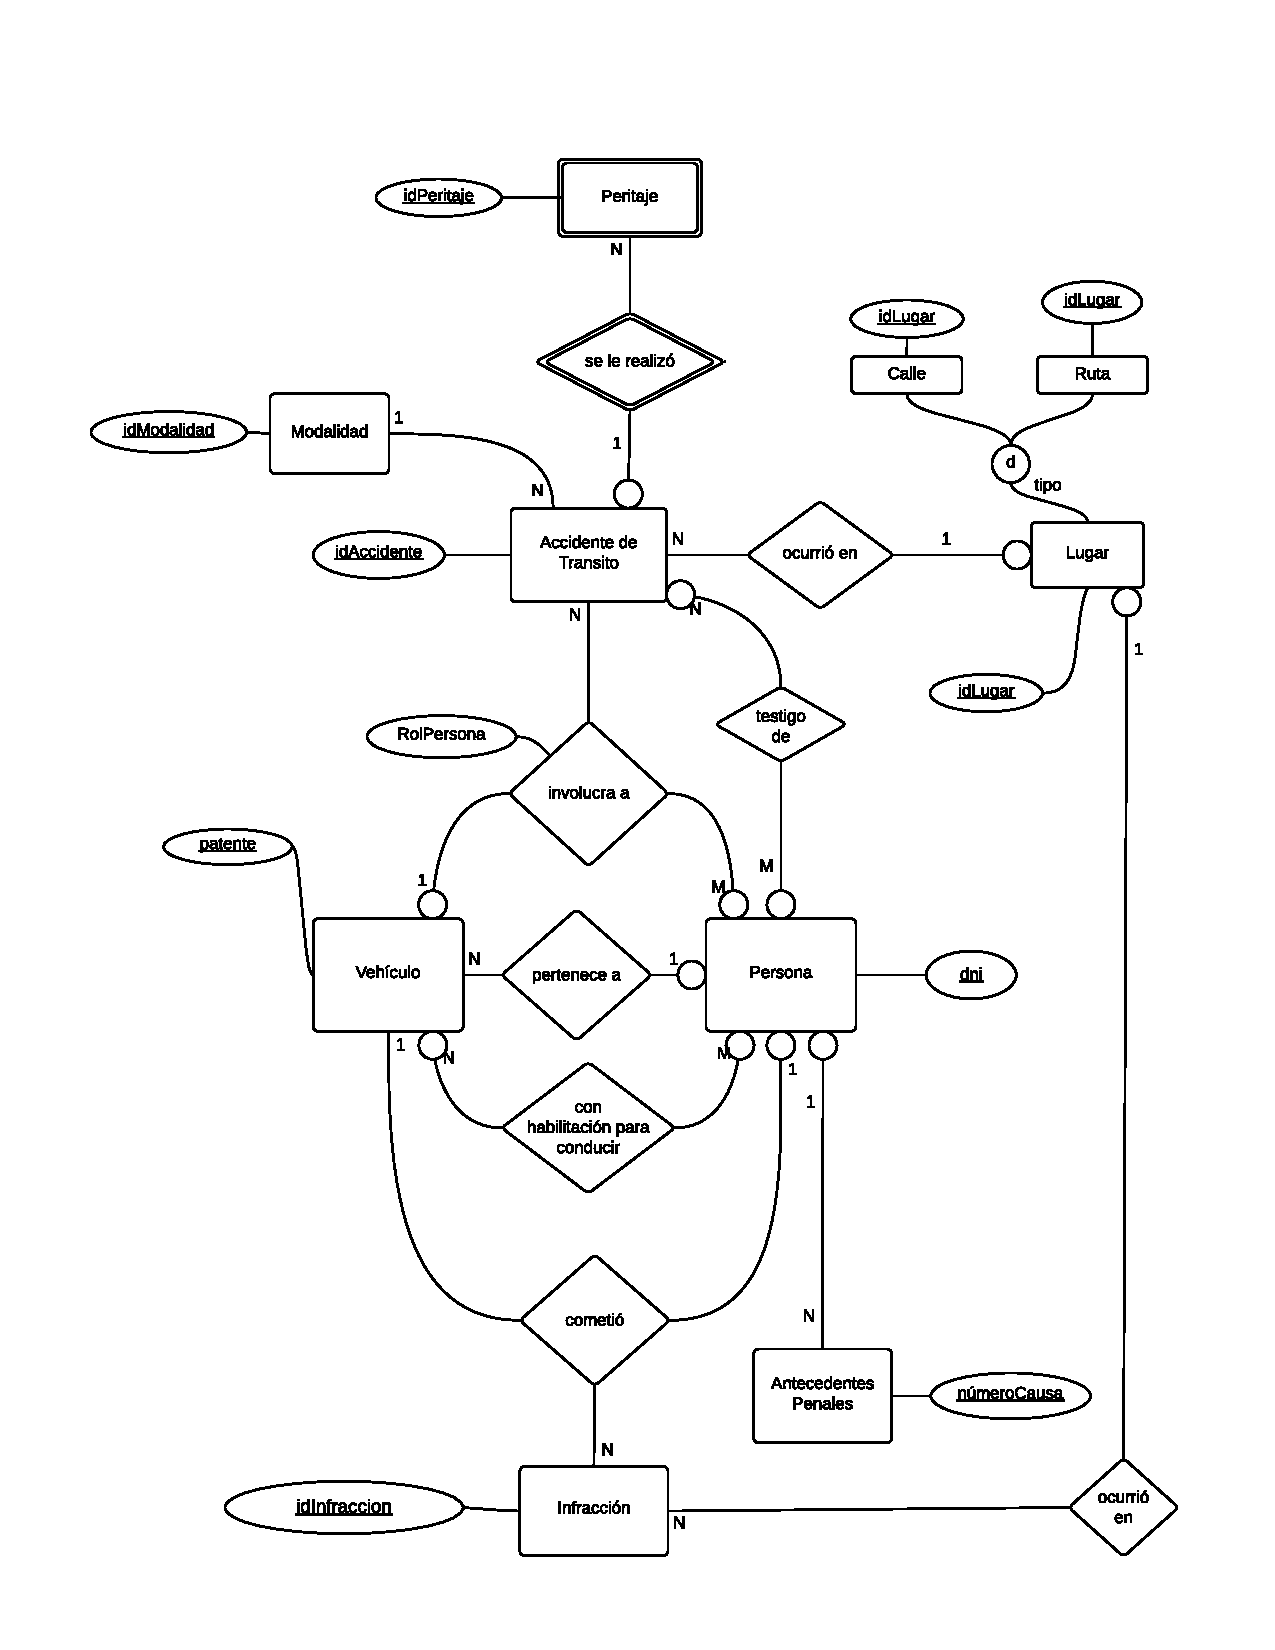
\includegraphics[scale=0.70]{diagramas/1.pdf}
    \caption{DER con PK's únicamente}
  \end{center}
\end{figure}

\subsection{Asunciones del dominio}

\begin{itemize}
  \item \textbf{DNI:} Todas las personas tienen DNI, y este es único para cada persona.
  \item \textbf{Lugar:} Los accidentes solo ocurren en calles y rutas. Por lo tanto se dividen en estas categorías(disjuntas).
  \item \textbf{Lugar:}  El tipo de pavimento de un lugar(calle o ruta) es uniforme a lo largo de toda su extensión.
  \item \textbf{Lugar:}  El tipo de pavimento de un lugar(calle o ruta) es uniforme a lo largo de toda su extensión. Es decir, no hay calles que estén asfaltadas en algunos tramos y no lo estén en otros.
  \item \textbf{Lugar:}  La velocidad máxima permitida de un lugar(calle o ruta) es uniforme a lo largo de toda su extensión.
  \item \textbf{Denuncias:}  Las denuncias policiales son tomadas por un único oficial.
  \item \textbf{Peritaje:}  Cada peritaje es realizado por un único perito.
  \item \textbf{Peritaje:}   Un peritaje consiste de un análisis de un factor relevante en el accidente. Por ejemplo, estado de iluminación de la vía al momento del accidente.
  \item \textbf{Peritaje:}  Cada peritaje tiene su resultado.
  \item \textbf{Accidente:}  Las personas tienen un único rol en un accidente: Pueden ser conductores o acompañantes de un vehículo, terceros afectados por este último o testigos. Los testigos no se relacionan con un vehículo en particular.
\end{itemize}

\subsection{DER con Primary Keys únicamente}
Como el diagrama está compuesto por muchas entidades con muchas relaciones, incluímos como primera aproximación un esqueleto
del modelo, en donde incluímos únicamente las entidades con sus claves primarias, la cardinalidad de las relaciones y
los atributos más relevantes.

\subsection{DER completo}
El diagrama completo fue separado en varias partes para facilitar su lectura.

\newpage
\begin{figure}
  \begin{center}
    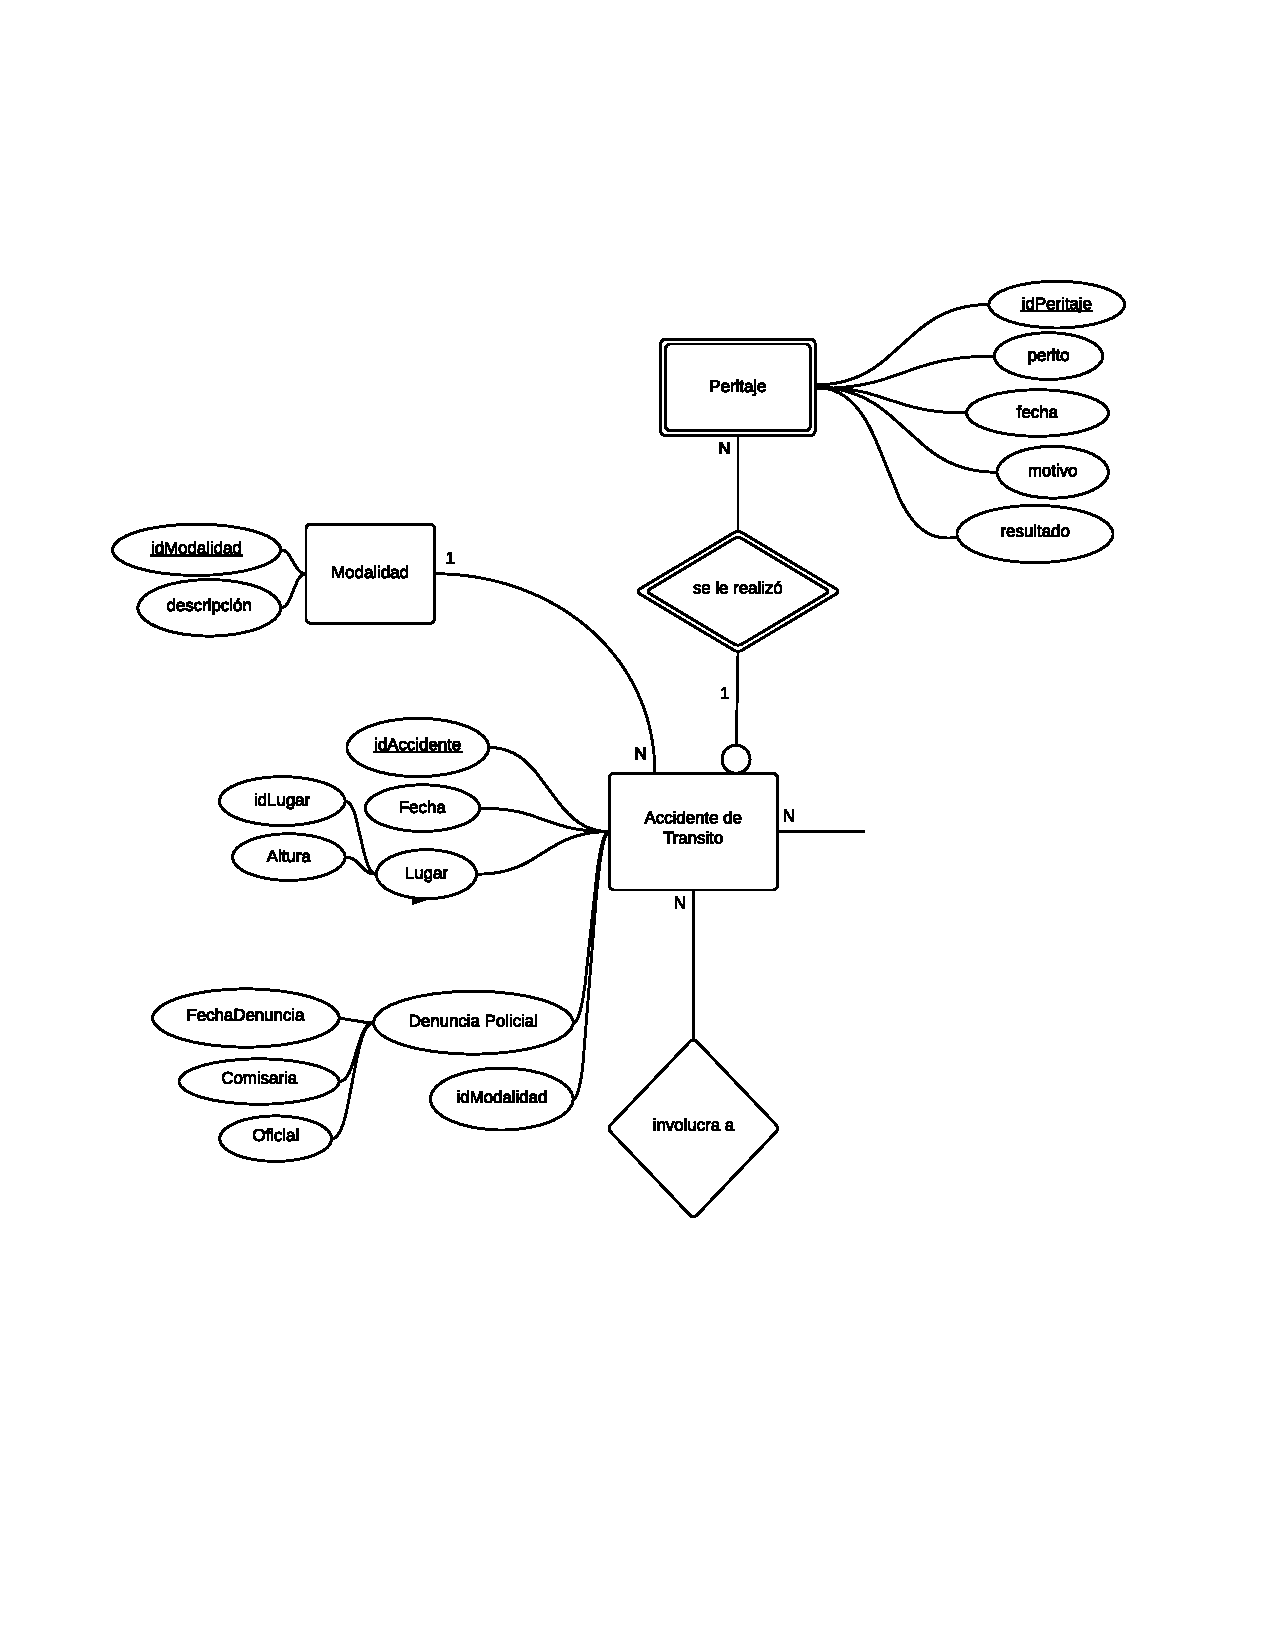
\includegraphics[scale=0.80]{diagramas/2-1.pdf}
    \caption{Accidente.Modalidad.Peritaje}
  \end{center}
\end{figure}

\newpage
\begin{figure}
  \begin{center}
    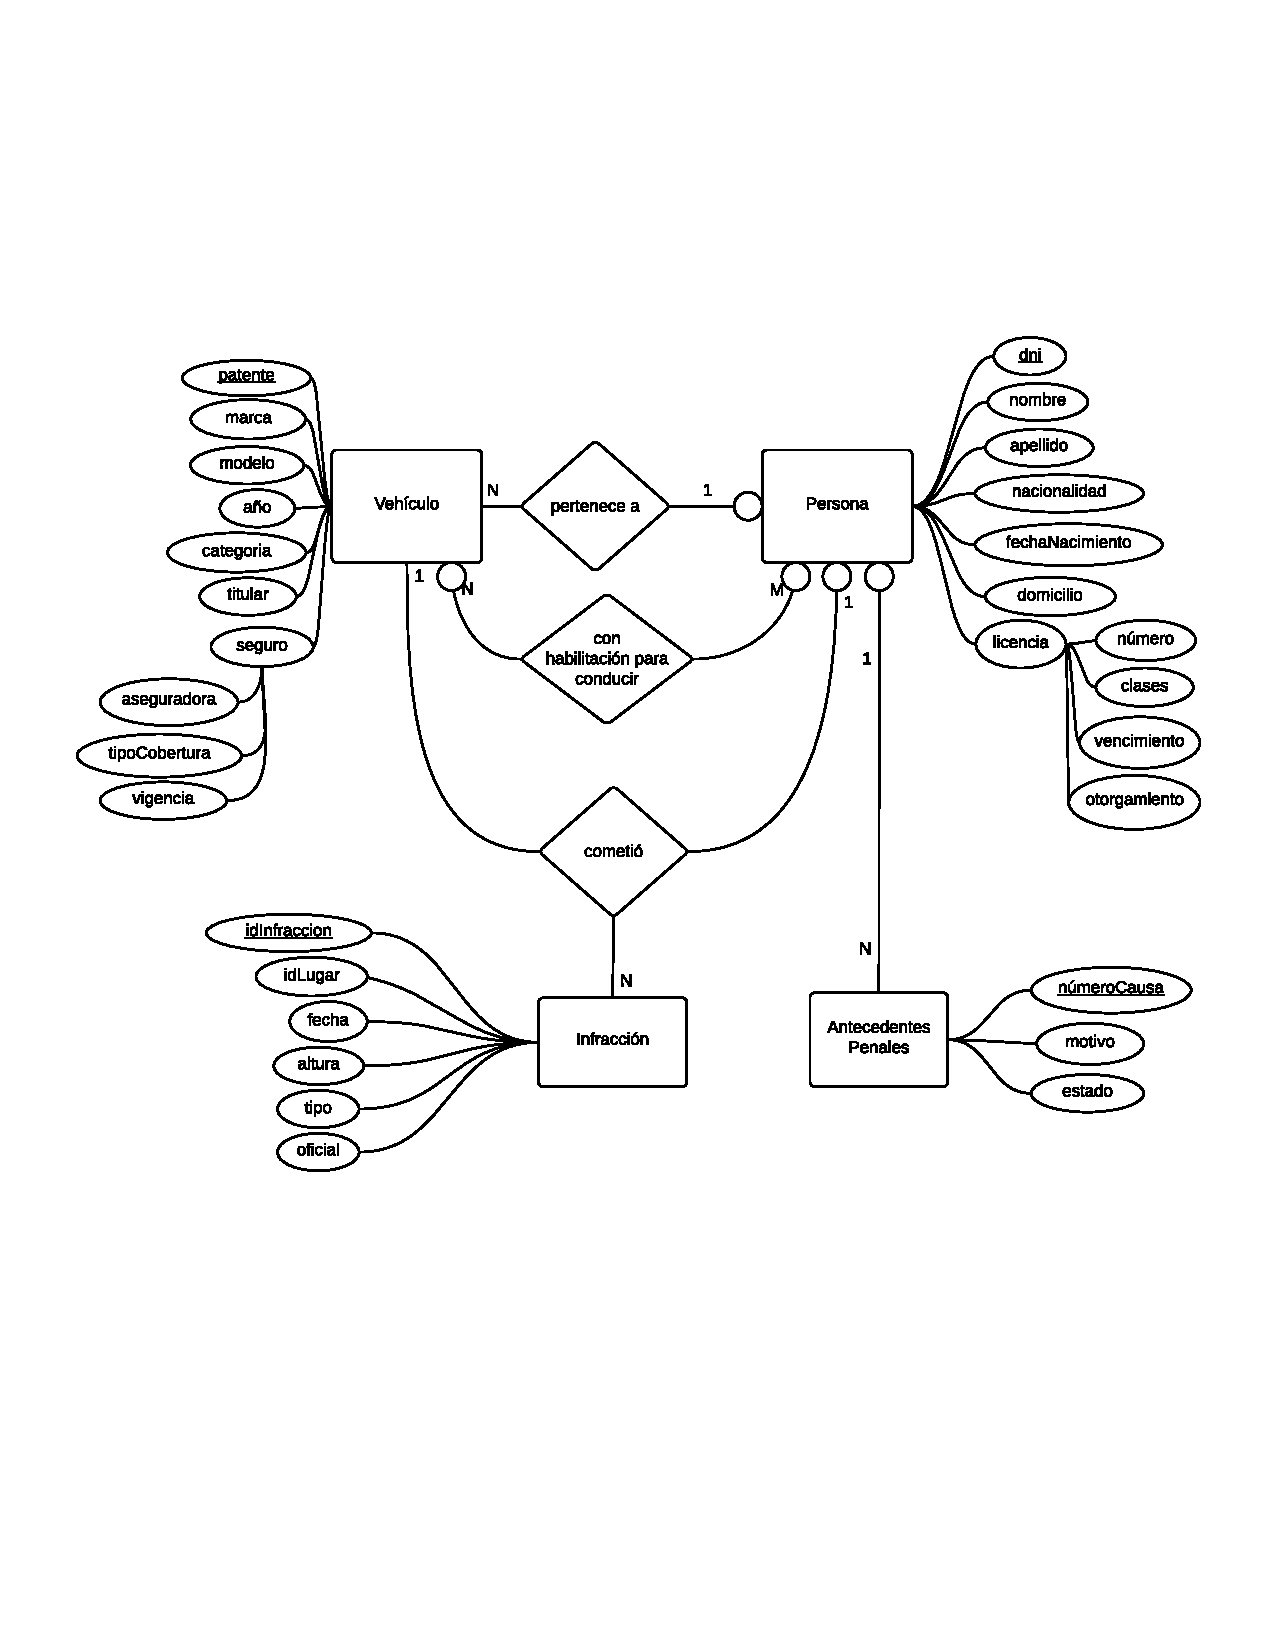
\includegraphics[scale=0.8]{diagramas/2-2.pdf}
    \caption{Vehículo.Persona.Antecedentes penales.Infracción}
  \end{center}
\end{figure}

\newpage
\begin{figure}
  \begin{center}
    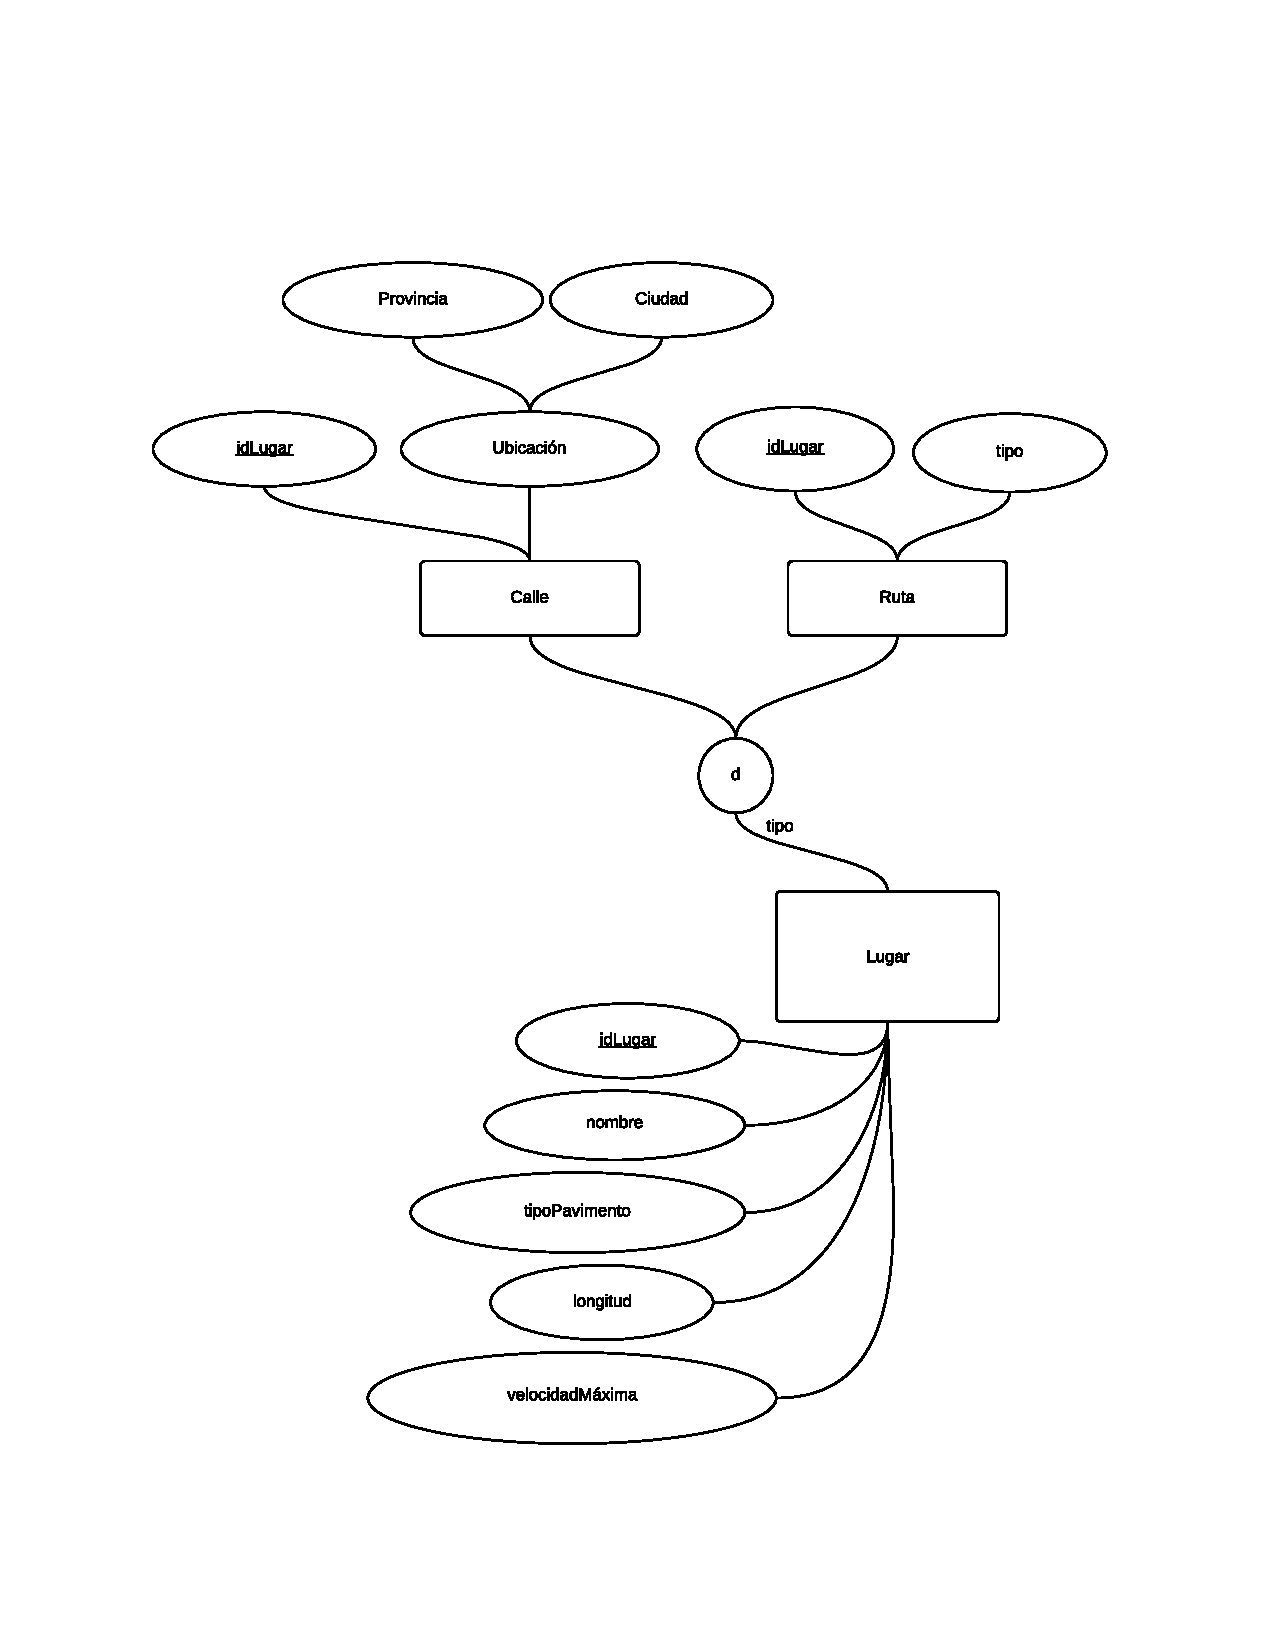
\includegraphics[scale=0.6]{diagramas/2-3.pdf}
    \caption{Lugar:Calle/Ruta}
  \end{center}
\end{figure}

\newpage
\begin{figure}
  \begin{center}
    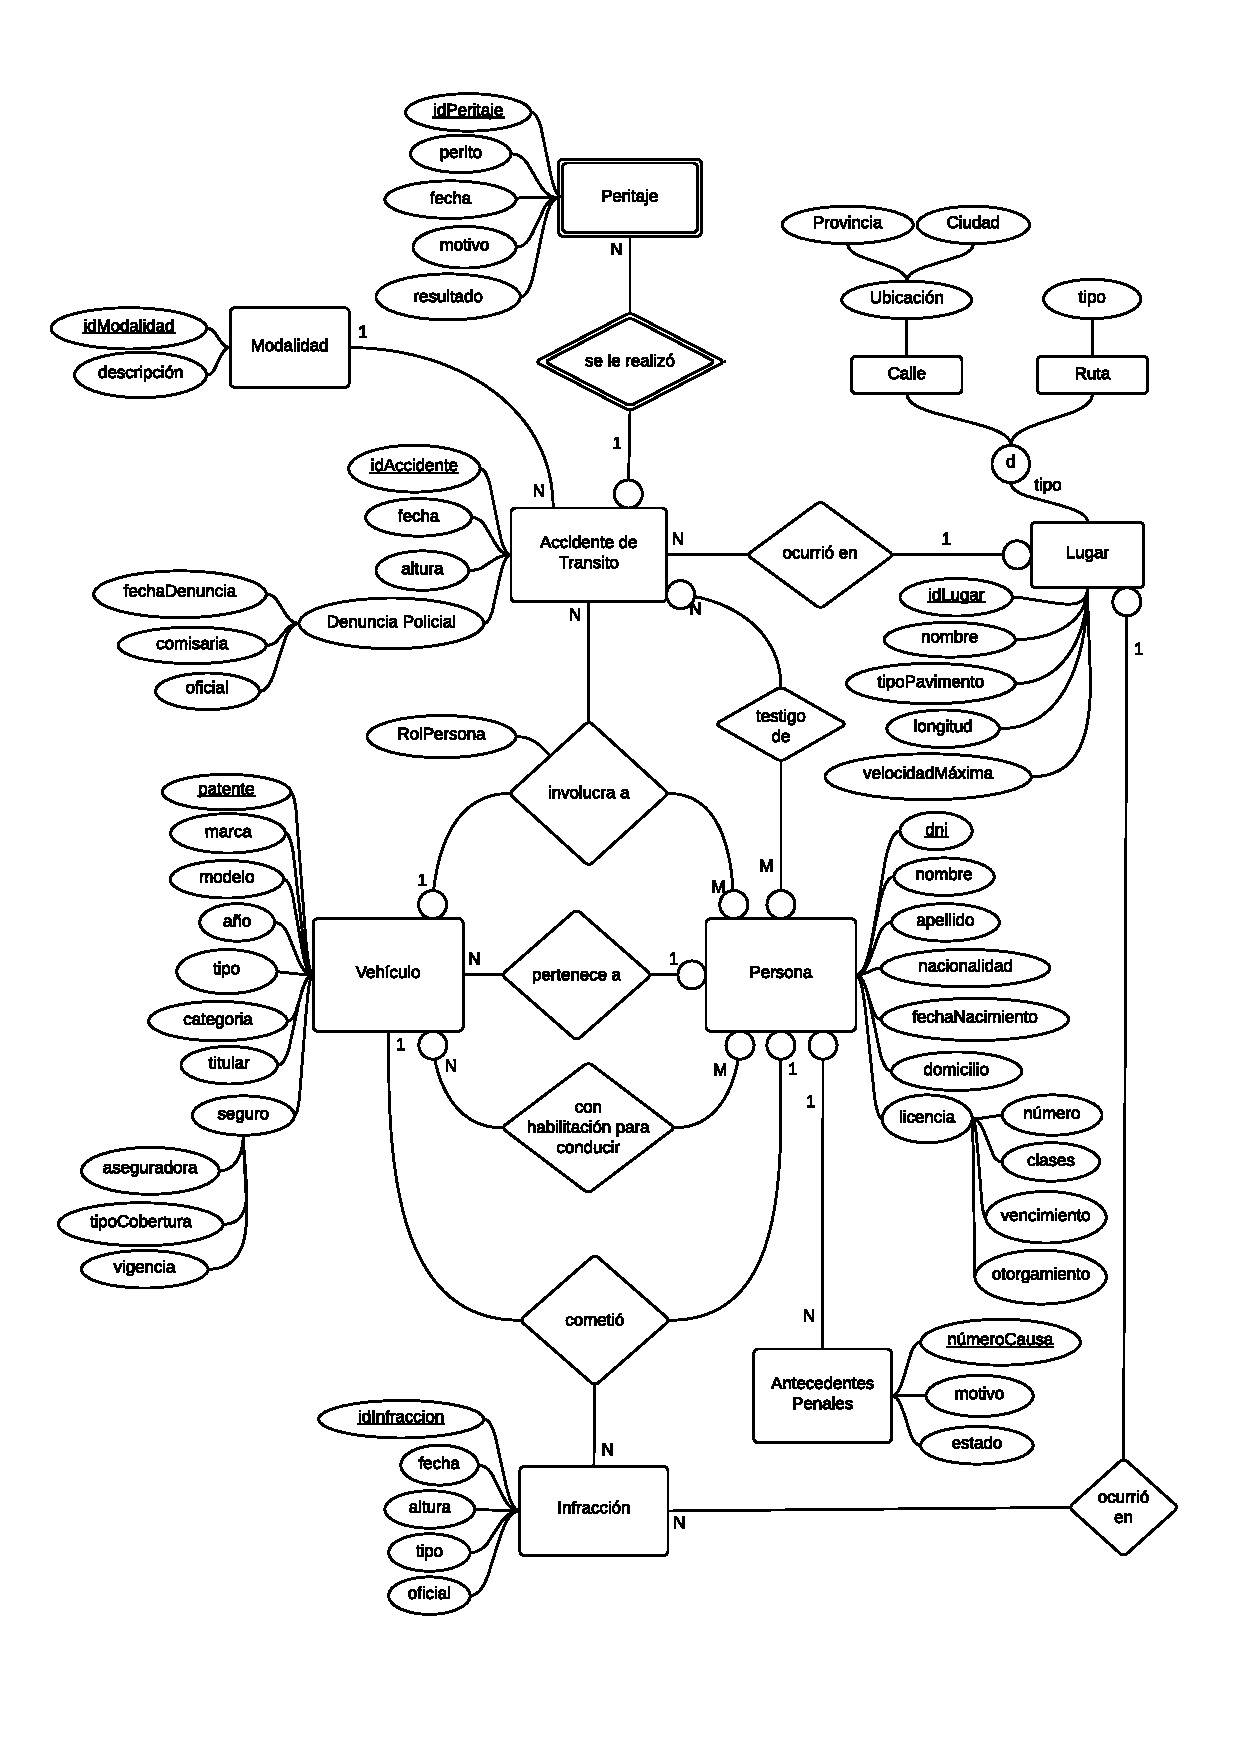
\includegraphics[scale=0.6]{diagramas/3.pdf}
    \caption{DER completo}
  \end{center}
\end{figure}


\newpage
\subsection{Reestricciones en lenguaje natural}

Cuestiones de notación: Cuando decimos que una entidad ''tiene'' un atributo, nos referimos a que dicho campo no puede ser \textbf{Null}.

\begin{enumerate}
  \item \textbf{Involucra_a:}
  \begin{enumerate}
    \item \textbf{Alguien manejaba y es único:} Dados un accidente y un vehículo involucrados en un accidente, existe una \underline{única} persona que manejaba ese vehículo en dicho accidente. Es decir, que tiene rol de conductor.
    \item \textbf{Conductores no son acompa\~nantes:} Las personas con rol de acompañante para un vehículo y un accidente no pueden estar involucrados como conductores de dicho vehículo en dicho accidente.
    \item \textbf{Conductores tienen licencia:} Las personas con rol de conductor de un vehículo en un accidente tienen licencia que les permite conducir ese vehículo.
    \item \textbf{Pasajeros no son testigos:} Las personas que están involucradas en un accidente y un vehículo no pueden ser testigos de los mismos.
    \item \textbf{Terceros afectados:} Los terceros afectados por un vehículo en un accidente no pueden ser conductores ni acompañantes en el mismo accidente.
    \item \textbf{Conductores tienen habilitación para conducir:} Si una persona conducía el vehículo en una accidente, entonces tiene habilitación para conducir ese vehículo.
  \end{enumerate}
  \item \textbf{Vehículo:}
    \begin{enumerate}
      \item \textbf{Tienen patente:} Todos los vehículos tienen patente, y ésta es única.
    \end{enumerate}
  \item \textbf{Peritaje:}
    \begin{enumerate}
      \item \textbf{Tienen motivo:} Los peritajes tienen descripción.
      \item \textbf{Tienen resultado:} Los peritajes tienen resultado.
      \item \textbf{Tienen fecha:} Los peritajes tienen fecha posterior a la del accidente.
      \item \textbf{Tienen perito:} Los peritajes son realizados por algún perito.
    \end{enumerate}
  \item \textbf{Denuncia:}
    \begin{enumerate}
      \item \textbf{Tienen denuncia:} Todos los accidentes tienen denuncia policial.
      \item \textbf{Denunciado en comisaría:} Las denuncias son hechas en una comisaría.
      \item \textbf{Realizada en una fecha específica:} Las denuncias son realizadas en una fecha. Ademàs, la fecha de la denuncia es igual o posterior a la fecha del accidente.
      \item \textbf{Acta labrada por un oficial:} El acta de las denuncias es labrada por un oficial.
    \end{enumerate}
\end{enumerate}





